\section{Umsetzung}
Hier noch generell was beschreiben. - Zielarchitekturbild darstellen (komplette Architektur)

\colorbox{yellow}{Hier fehlt was}

\begin{figure}[h]
    \centering
    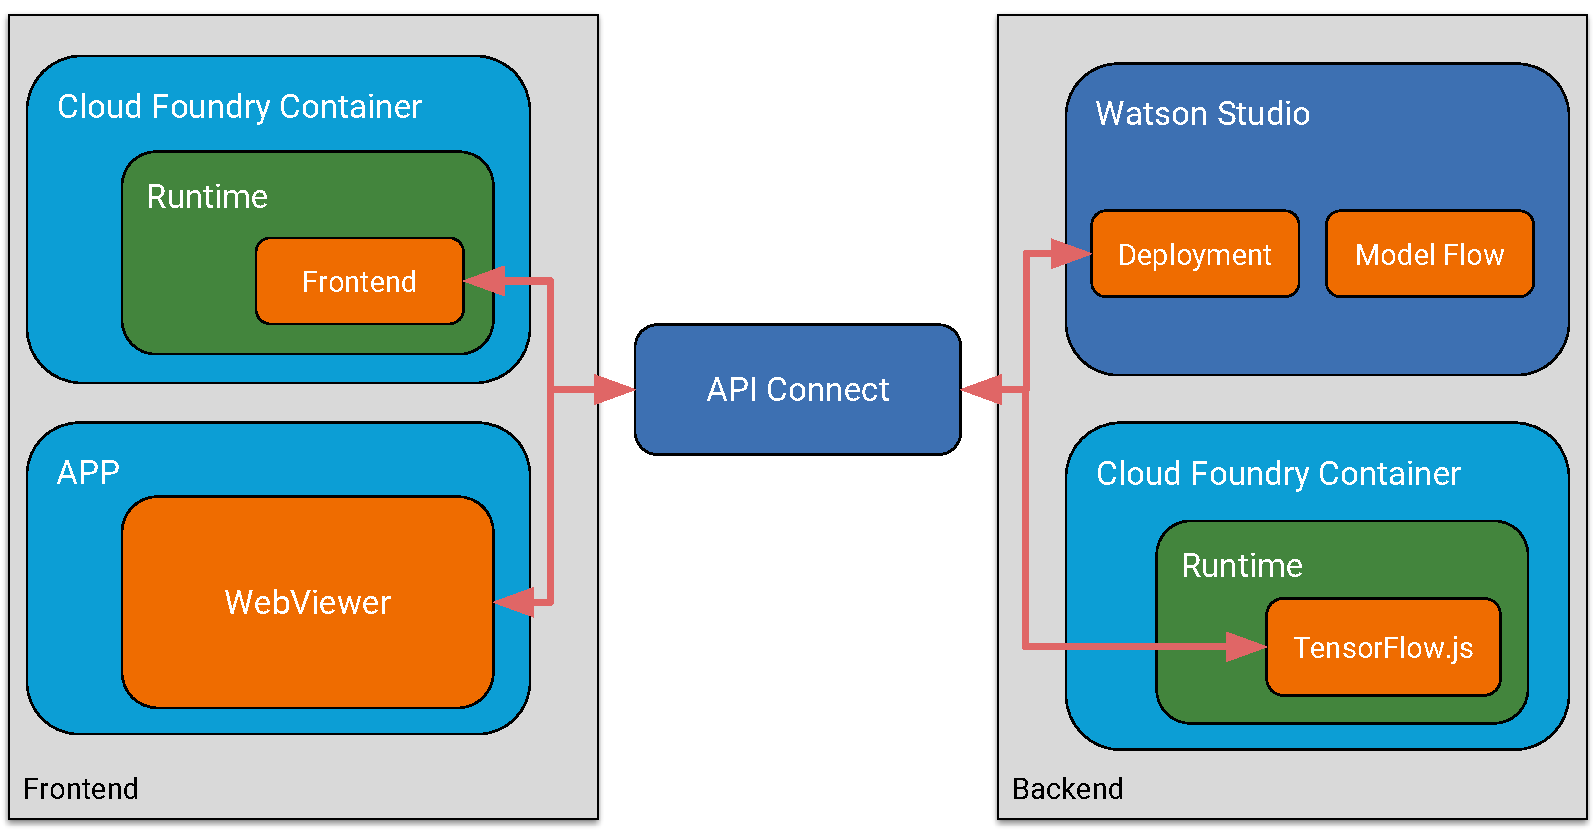
\includegraphics[width=\textwidth]{images/kapitel_4/architektur_uebersicht.pdf}
    \caption{Übersicht über die Zielimplementierung}
    \label{fig:umsetzung_zielarchitektur_4}
\end{figure}

\subsection{Webseite}
\label{subsec:webseite}
Bauen und erstellen der eigentlichen Webseite
Mockups werden auch erstellt. Wie sehen die aus etc.

\begin{figure}[h]
    \centering
    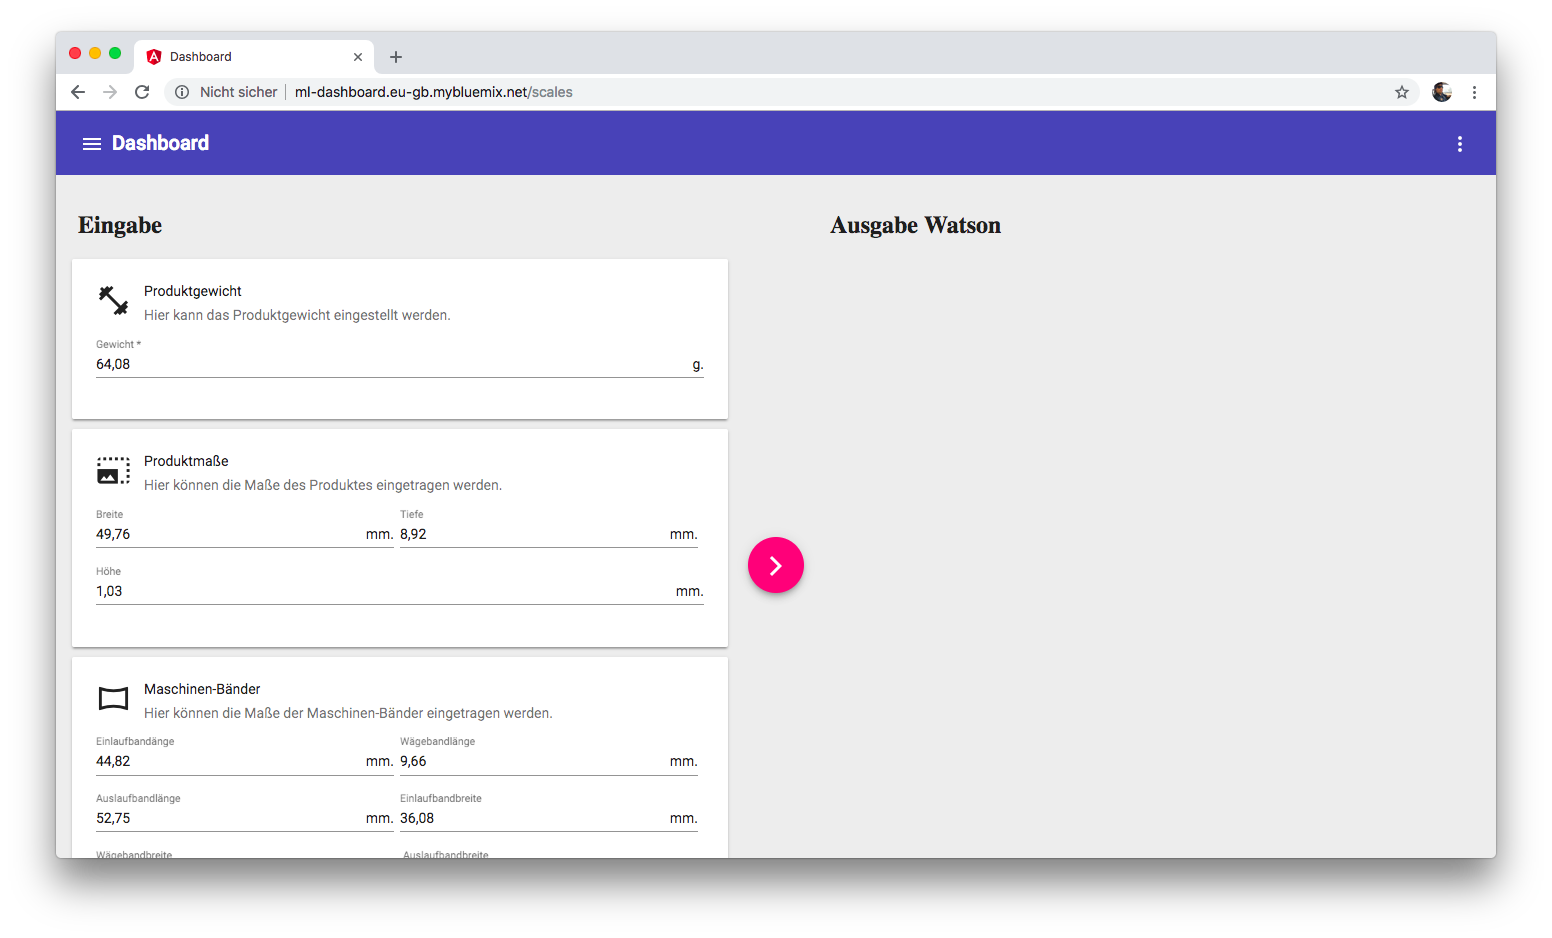
\includegraphics[width=\textwidth]{images/kapitel_4/website_input.png}
    \caption{Kompletter Model flow}
    \label{fig:umsetzung_website_input}
\end{figure}

\begin{figure}[h]
    \centering
    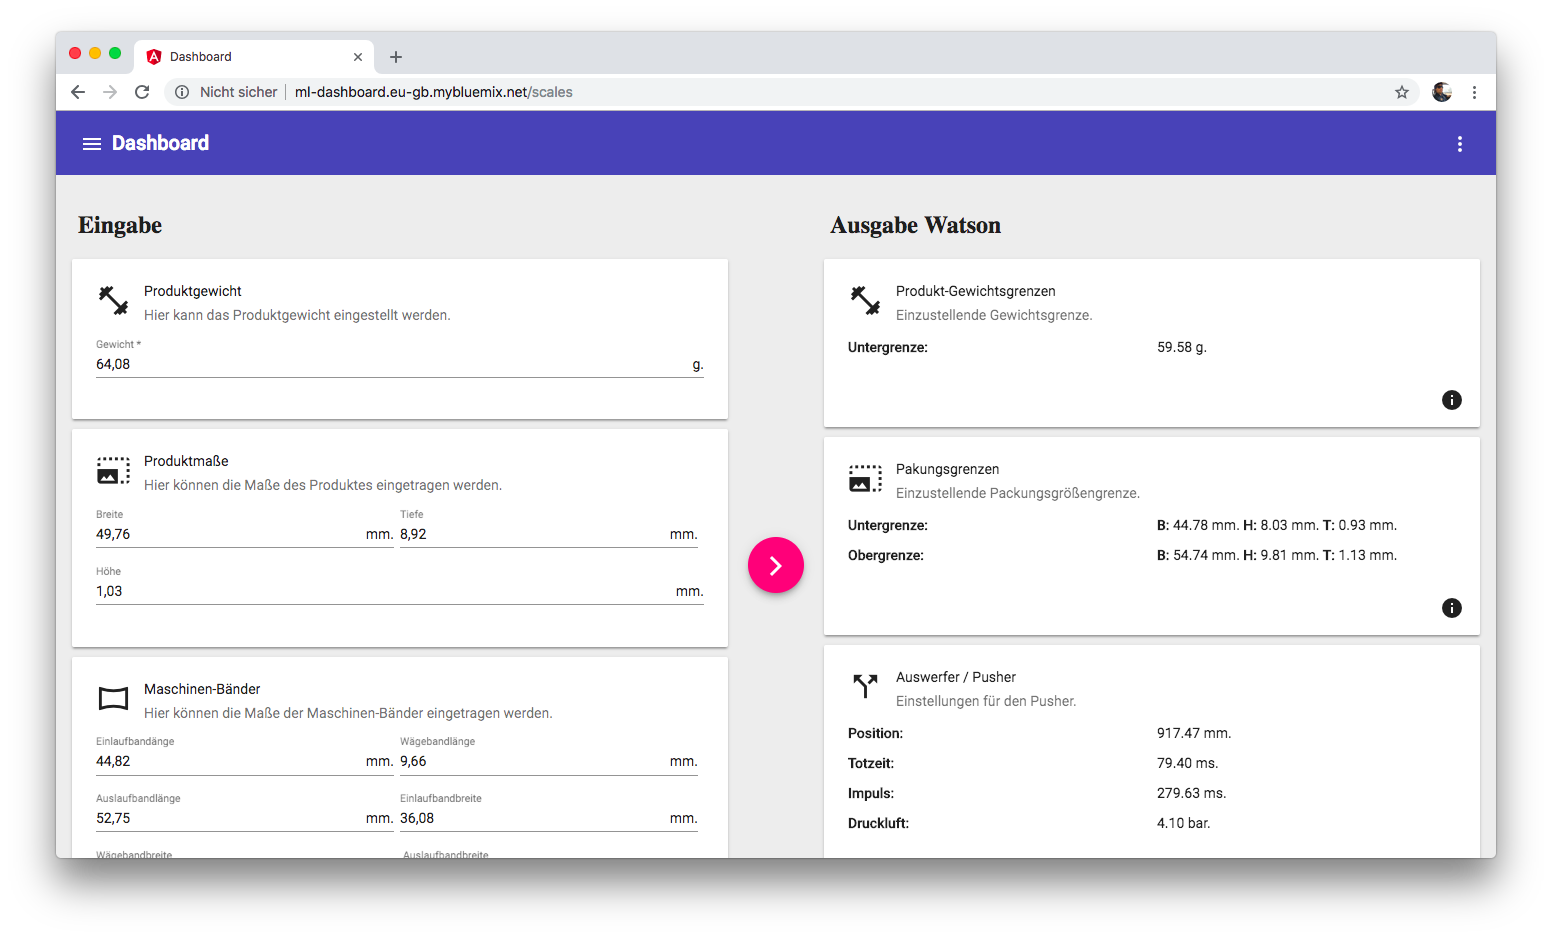
\includegraphics[width=\textwidth]{images/kapitel_4/website_output.png}
    \caption{Kompletter Model flow}
    \label{fig:umsetzung_website_output}
\end{figure}

\colorbox{yellow}{Hier fehlt was}

\subsubsection{Mockups erstellen}
\colorbox{yellow}{Hier fehlt was}

\subsubsection{Webseite umsetzen}
\colorbox{yellow}{Hier fehlt was}

\subsubsection{Offline-Mode}
\colorbox{yellow}{Hier fehlt was}

\subsubsection{Toolchain einrichten}
\colorbox{yellow}{Hier fehlt was}

\subsection{Smartphone App}
Hier muss ein bisschen Beschreibung hin.

\colorbox{yellow}{Hier fehlt was}

\subsubsection{Android}
Bauen und erstellen der Apps

\colorbox{yellow}{Hier fehlt was}

\subsubsection{iOS}
Bauen und erstellen der Apps

\colorbox{yellow}{Hier fehlt was}